\documentclass[10pt, conference, compsocconf]{IEEEtran}
\usepackage{amsmath}  
\usepackage{graphicx}
\hyphenation{op-tical net-works semi-conduc-tor}
\begin{document}

\title{Travelling Salesman Problem}
\author{\IEEEauthorblockN{Christopher Parker}
\IEEEauthorblockA{Biologically Inspired Computing\\
University of Oslo\\
Fall 2014\\
%Huntsville, Alabama\\
%chris@chris-parker.net
}
}
\maketitle


\begin{abstract}
Three search techniques are applied to the travelling salesman problem (TSP) are considered: exhaustive, greedy, \& genetic algorithm. The exhaustive search is found to be unfeasible for modest problem sizes. Greedy search (hill climbing) performs well over small run times, but is ultimately outperformed by genetic search. Genetic search performance is found to vary $negatively$ with population size. This is attributed to proportionally increased generation run time. Stochastic 2-opt (subsequence reversal) was found to be the best operator for both genetic mutation and greedy search.

The relevant code \& example output images may be found at: 

\centerline{github.com/csp256/INF3490\_Homework\_1}
\end{abstract}

%\begin{IEEEkeywords}
%Travelling salesman, genetic algorithm, hill climbing, exhaustive search, Python, matplotlib
%\end{IEEEkeywords}
\IEEEpeerreviewmaketitle


\section{Introduction}
The travelling salesman problem (TSP) is an NPO-complete problem with many important real-world applications, such as lithography, network load balancing, transportation infrastructure, and many others. Unfortunately, it can not be solved exactly for practical problem sizes. Optimization heuristics must instead be employed to generate a, hopefully sufficiently optimal, approximate solution.

This paper considers the behavior of three such search heuristics: exhaustive search, hill climbing, and genetic search. Each of these search techniques are given a specified, finite amount of time to return the best possible answer. This time-limited feature is why exhaustive search is herein classified as a heuristic. 


\section{Theory \& Algorithm Specification}
All comparisons in this paper are given in terms of run time, not search iterations. This is because each heuristic does significantly different amounts of computation per each iteration. It is simply not a meaningful comparison to compare the fitness of a genetic search with population N to a genetic search with population M$\neq$N, in a compute limited (or serial) environment. The ability to perform suitably well under resource constraints is also considered to be a more important characteristic of search heuristics than their performance per generation.

\subsection{Paths and Lengths}
A path, also called a tour, is a permutation of all $n$ vertices in a subgraph of order $n$. In the scope of this project $n=\{10,\,24\}$ and the subgraph is fully connected, directed, and symmetric. Presumably, it also satisfies the triangle inequality on $L_2$, but this additional information was not verified or exploited. 

The path length is the sum of the weights of all adjacent vertices in the path, including the edge from the last to the first vertex. Accordingly, cyclic permutations and reflections of a path are of identical length. Because there are $n!$ paths, there are therefor, at most $\frac{(n-1)!}{2}$ unique path lengths.

All reported "logarithmic path lengths" or "logarithmic fitness" values are given as the natural logarithm of the actual path length. Please also be aware that the "percent completed" metric on earlier graphs is two orders of magnitude too small due to an error.

\subsection{Exhaustive Search}
Python provides a function to enumerate all permutations of a list. This is not used, due to its $n!$ memory complexity. Instead, a function similar to the Fisher shuffle algorithm imposes an implicit enumeration (and ordering) to the set of all permutations and permits the generation of a specific member of the set of all permutations without the the computation of other permutations. It is $O(1)$ in memory and roughly linear in time.

This search technique proceeds wholly uninformed. In a sense it represents the "worst" search algorithm.

\subsection{Greedy Search (Hill Climbing)}
The greedy search algorithm starts with a single random state. It then generates a "similar" state and sets it as the current state if it is better. The process iterates. 

Herein the similar state is chosen to be stochastic subsequence reversal. This is similar or equivalent to the 2-opt procedure discussed in the literature. The subsequence position is uniformly distributed, and the length is generated from a modified normal distribution plus a constant of $2$ to prevent trivial . The modified normal distribution is the floor (truncate to zero) of the magnitude of the normal distribution with mean $0$. The variance of this distribution is chosen to be one fifth of the order $n$ of the subgraph. This was chosen so that smaller subsequences will be reversed more frequently, and subsequences larger than one half the order of $n$ almost never occur (these subsequences are exactly equivalent to their compliment). 

The logarithm of the best tour length of greedy search is approximately a Pareto distribution as a function of time. However, it can become permanently stuck in local optima. Extensions to n-opt, v-opt, or simulated annealing techniques are the logical solution to this problem, but were not implemented. 

\subsection{Genetic Search}
In the genetic search heuristic, a population of $k$ candidate solutions are stored. They are recombined and mutated (altered stochastically) to generate a seperate set of $k$ new candidate solutions, in analogy to sexual reproduction. Each solution is paired with another solution from the other pool. One of these pairs is discarded and the process iterates. These processes are carried out so that the entire population's fitness tends to improve over time, where fitness is determined here to be a function of the path length.

For the creation of each new candidate solution, two potential new 'child' solutions are generated from two previous 'parent' solutions. Each parent is chosen from draw-2-choose-1 tournament selection. Duplicates are permitted. For each sequential number $i$ from $[1,n]$, a fair coin is flipped. If it is heads, the first parents $i^{th}$ vertex is appended to the first child. Elsewise, the second parents corresponding vertex is appended to the second child. Afterwards, vertices not included in the first childs path are added, in order, from the second parent (and similarly from the first parent to the second child). For each child, with some small probability, the child is mutated (transformed) into a nearby solution, using the same definition of 'nearby' as found in the greedy search. Finally, the less fit child is discarded.

Initial population generation is performed by uniform sampling of the space of possible tours. 

\section{Results}
Parameters of several types were considered, but those relevant to this paper are all combinations of graph order $n=\{10,\,24\}$, population size $k=\{\frac{n}{4},\,\frac{n}{2},\,n\}$ (also known as the "population multiplier" since it is a function of the graph order $n$), run time $t=\{0.01s,\,0.03s,\,0.1s,\,0.3s,\,1s,\,3s,\,10s\}$, and number of search iterations $i=\{20\}$.

\subsection{Exhaustive Search}
Exhaustive search takes 30$\pm$5 seconds to complete for $n=10$, and finds the optimal path of length 7486.31. Thermodynamic limitations on computation possible in our Universe prevent it from converging for $n=24$. In the alotted time available to the other search methods, it explores a vanishingly small portion of the search space that is similarly appropriate for astrophysical metaphor. 

\subsection{Greedy Search}
Greedy search performs very well over the considered problem size and time limits. It completed ~170,000 iterations per second and shows early growth that is more rapid than genetic search, but is slower after "low hanging fruit" has been exploited.  

For $n=10$ more than 95\% of greedy search iterations converged to the global optimum. However, this does not imply all such searches converge. For $t=30$, one search iteration was found to become stuck in a local optimum for ~27 seconds until the algorithm terminated.

\subsection{Genetic Search}
Of 4 considered mutation probabilities $P=\{0.02,\,0.2,\,0.5,\,1.0\}$, $P=0.02$ consistently created the most desirable average and best solutions with $t=1,\,n=24,\,i=20$. 

Two types of mutation were implemented: the subsequence reversal heuristic (identical to greedy search's candidate generation), and a method based on the Fisher shuffe. The latter technique performed a cyclic permutation of the path, transformed the result by a random but relatively low-index call to the permutation generation function used in exhaustive search, and then reversed the cyclic permutation. This served to inject a large amount of entropy into a small random subsection of the path. Inclusion of this technique was found to behave worse in every case, likely due to implementation performance, and was subsequently disabled.

Larger population sizes universally performed worse (due to computation cost per generation) except for when the run time relative to the problem size was large. The additional diversity from a large population seems to increase consistency and resiliency in exchange for slower convergence per unit time.

The performance issue of the genetic search is most obvious when you recognize that only ~40\% as many solutions are generated per unit time as greedy search. Despite this limitation, genetic search outperforms greedy search for large $n$ and $t$: in a run of $n=24,\,t=180$ greedy search found a path with length 19046, while genetic search ($k=\frac{n}{4}$) found a path with length 13855. For contrast, exhaustive search found a path with length 21589.

\section{Future Work}
The hill climbing algorithm can become stuck in local optima. Extending the algorithm to include to n-opt, v-opt, simulated annealing, or random restart techniques is the logical solution to this problem.

The genetic algorithm suffers from performance issues. Additional (and more general) crossover, mutation, and selection operators are desirable. Lamarckian and Baldwinian learning is an obvious next step.

Many parts of this code can, and should, be parallelized. Unfortunately, it is implemented in Python.

The entire code base needs to be refactored to use an object oriented approach. While this was not originally necessary, the inclusion of graphing obviated the need for OOP even in projects as small as 500 LOC. Graphing also fails for long runs, even when the graphed data is constrained to be less that of short runs.

A database with more than 24 cities is desirable.

\section{Conclusion}
Exhaustive search should be used only for small order graphs. Greedy search performs best under strict time limits. Genetic search, as implemented here, has the best formance over longer time scales for larger problems. It is advisable to keep the population of this implementation as small as possible (for while it is implemented on a serial architecture).

%A vast number of other alternative approaches exist, and the statements in the previous paragraph are only valid within the constraints of this project.


\newpage
\begin{center}
Greedy Search\\
\begin{tabular}{l*{6}{c}r}
$n$&$t$    &\vline&  Best & Worst &  Mean & $\sigma$\\
\hline
\hline
10 & 0.1   &\vline&  7486 &  7871 &  7709 & 101 \\
   & 0.3   &\vline&  7486 &  7729 &  7560 & 89 \\
   & 1.0   &\vline&  7486 &  7664 &  7502 & 40 \\
\hline 
24 & 0.1   &\vline& 21315 & 23822 & 22442 & 711 \\
   & 0.3   &\vline& 20549 & 22954 & 22062 & 679 \\
   & 1.0   &\vline& 20018 & 21983 & 21903 & 585 \\
\end{tabular}
\end{center}
%\newpage
%$ $
%\newpage

$ \\
 \\
 \\
 \\
 \\
$
\begin{center}
Genetic Search\\
\begin{tabular}{l*{6}{c}r}
$n$&$t$  & Population Multiplier  &\vline&  Best & Worst &  Mean & $\sigma$\\
\hline
\hline
10 & 0.1 & 0.25 &\vline&  7486 &  8347 &  7572 & 258 \\
   &     & 0.5  &\vline&  7486 &  7486 &  7486 &   0 \\
   &     & 1.0  &\vline&  7486 &  7729 &  7545 &  84 \\
   & 0.3 & 0.25 &\vline&  7486 &  8391 &  7532 & 197 \\
   &     & 0.5  &\vline&  7486 &  8347 &  7529 & 188 \\
   &     & 1.0  &\vline&  7486 &  7486 &  7486 &   0 \\
   & 1.0 & 0.25 &\vline&  7486 &  8391 &  7620 & 318 \\
   &     & 0.5  &\vline&  7486 &  7486 &  7486 &   0 \\
   &     & 1.0  &\vline&  7486 &  7486 &  7486 &   0 \\
\hline 
24 & 0.1 & 0.25 &\vline& 19693 & 23933 & 21709 &1046 \\
   &     & 0.5  &\vline& 20428 & 23803 & 22288 & 839 \\
   &     & 1.0  &\vline& 20265 & 25449 & 23356 &1180  \\
   & 0.3 & 0.25 &\vline& 18578 & 21646 & 20088 & 789 \\
   &     & 0.5  &\vline& 18906 & 22412 & 20759 & 965 \\
   &     & 1.0  &\vline& 20699 & 23119 & 21807 & 624 \\
   & 1.0 & 0.25 &\vline& 17656 & 20217 & 18931 & 604 \\
   &     & 0.5  &\vline& 18218 & 20875 & 19798 & 655 \\
   &     & 1.0  &\vline& 19128 & 21692 & 20372 & 700 \\
\end{tabular}
\end{center}

\newpage
$ $
\newpage
\begin{figure}[t]
  \centering
    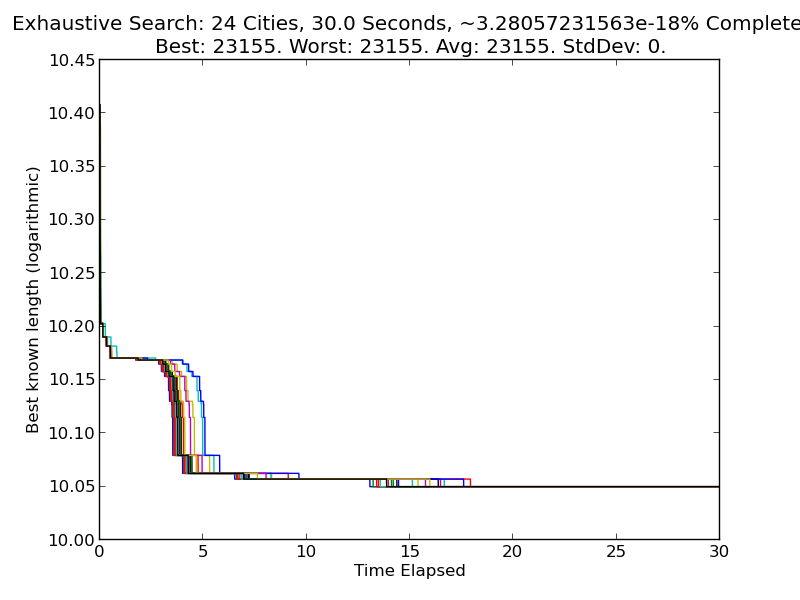
\includegraphics[width=1\textwidth]{../Example_Output_Images/24_cities/30_seconds/exhaustiveSearch.png}
\end{figure}
$ $


\newpage
$ $
\newpage
\begin{figure}[t]
  \centering
    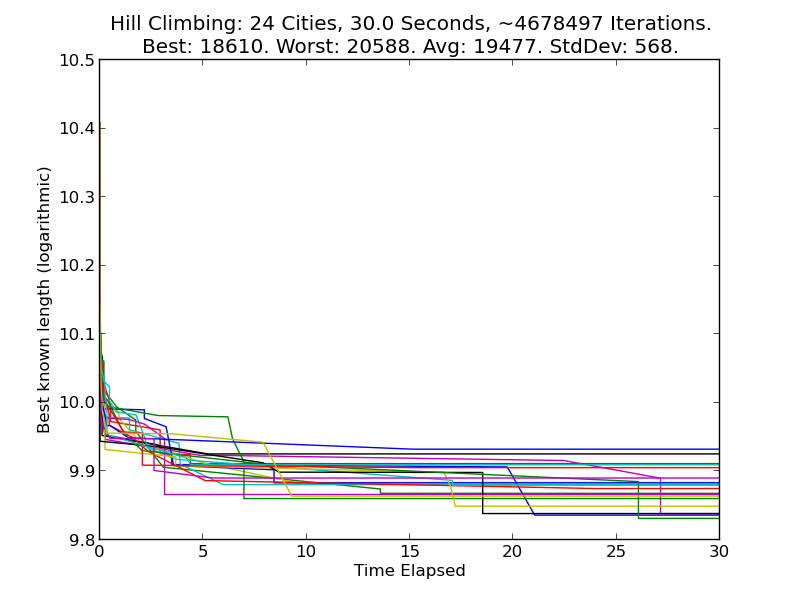
\includegraphics[width=1\textwidth]{../Example_Output_Images/24_cities/30_seconds/hillClimbing.png}
\end{figure}
$ $


\newpage
$ $
\newpage
\begin{figure}[t]
  \centering
    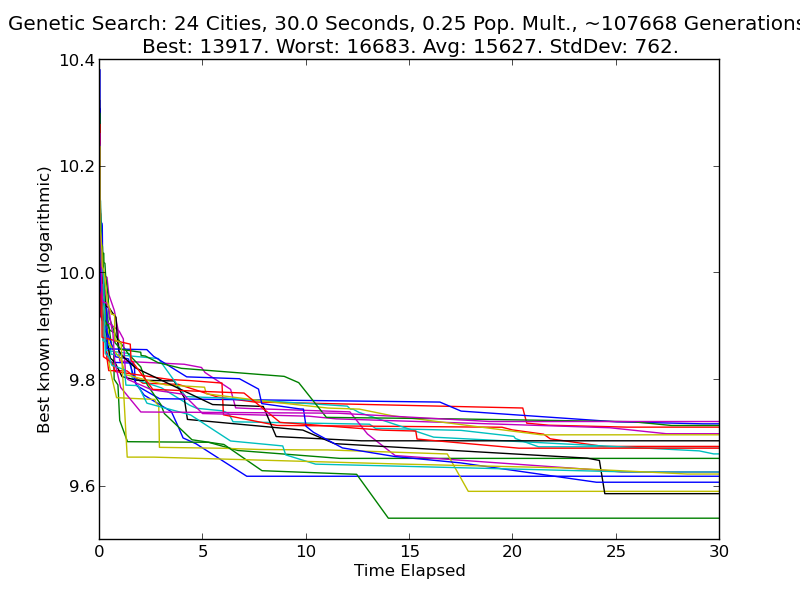
\includegraphics[width=1\textwidth]{../Example_Output_Images/24_cities/30_seconds/geneticSearch_025_populationMuliplier.png}
\end{figure}
$ $


\newpage
$ $
\newpage
\begin{figure}[t]
  \centering
    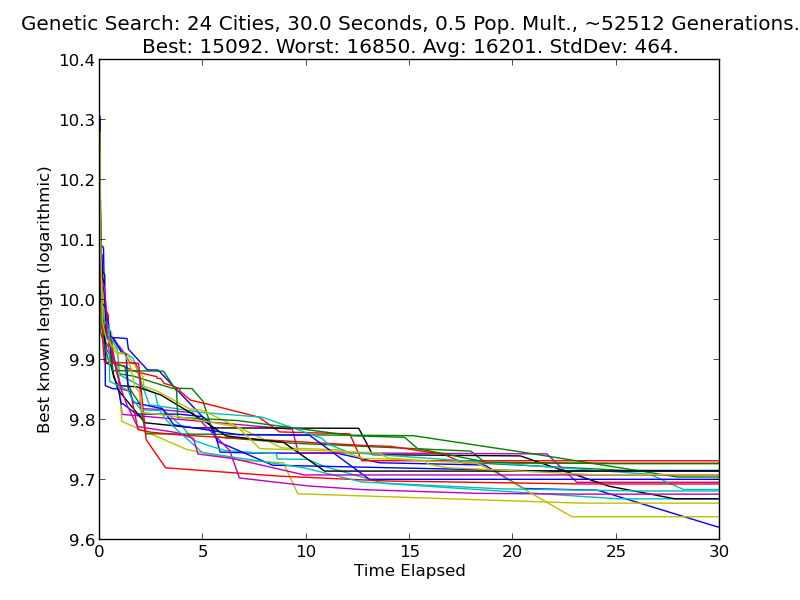
\includegraphics[width=1\textwidth]{../Example_Output_Images/24_cities/30_seconds/geneticSearch_05_populationMuliplier.png}
\end{figure}
$ $


\newpage
$ $
\newpage
\begin{figure}[t]
  \centering
    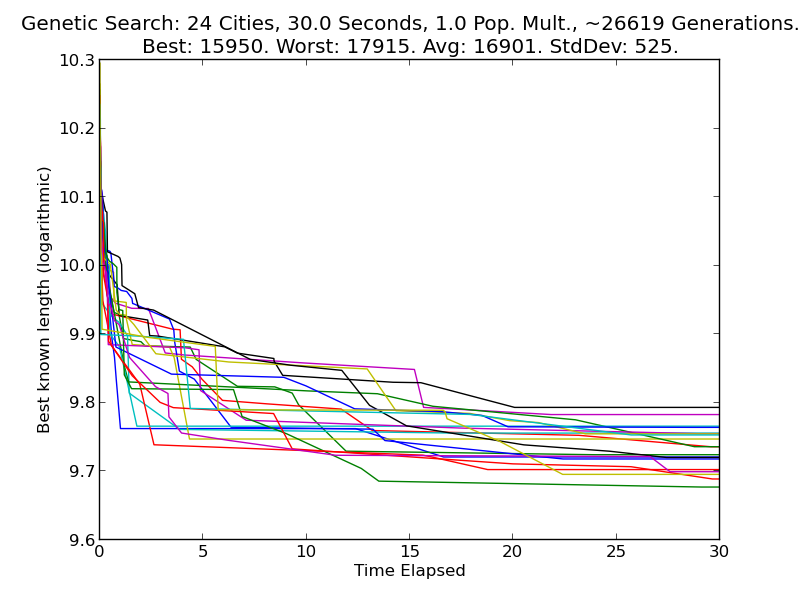
\includegraphics[width=1\textwidth]{../Example_Output_Images/24_cities/30_seconds/geneticSearch_10_populationMuliplier.png}
\end{figure}
$ $


\newpage
$ $
\newpage
\begin{figure}[t]
  \centering
    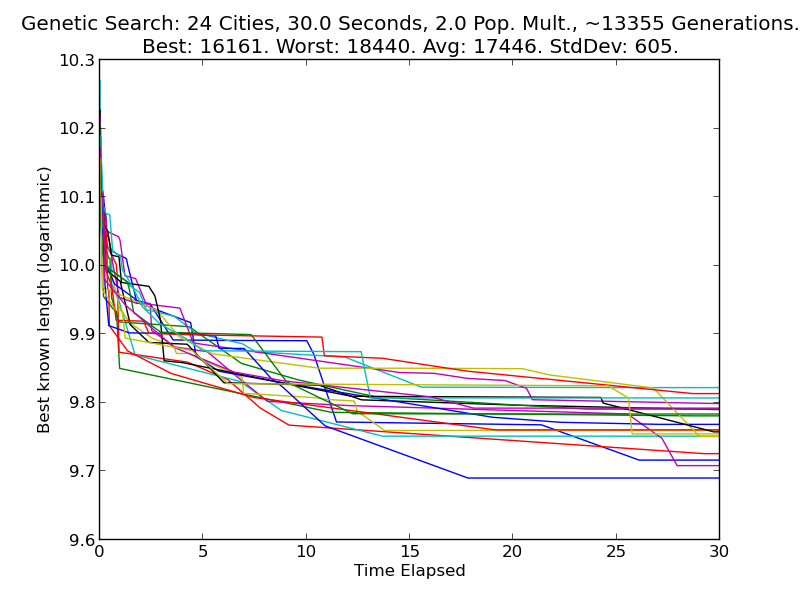
\includegraphics[width=1\textwidth]{../Example_Output_Images/24_cities/30_seconds/geneticSearch_20_populationMuliplier.png}
\end{figure}
$ $


\newpage
$ $
\newpage
\begin{figure}[t]
  \centering
    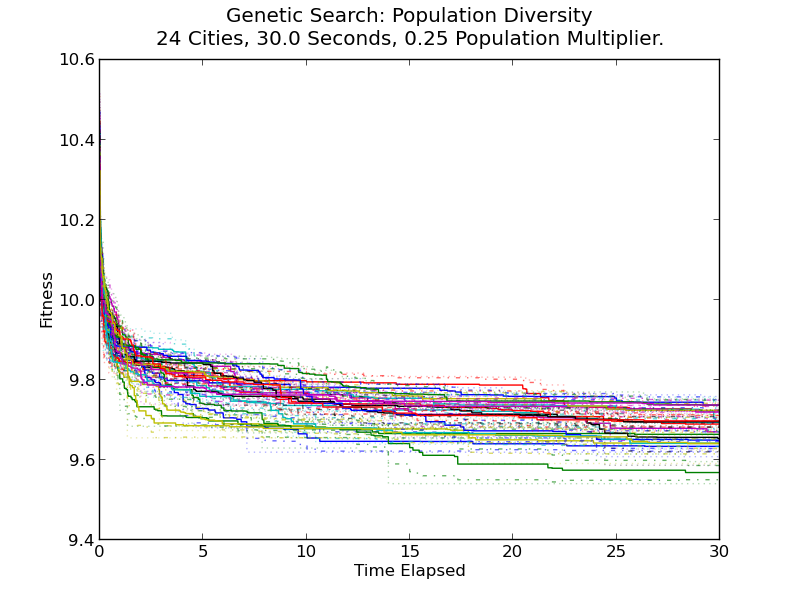
\includegraphics[width=1\textwidth]{../Example_Output_Images/24_cities/30_seconds/populationDiversity_025_populationMuliplier.png}
\end{figure}
The mean is representated as a solid line. The mean $\pm\sigma$ is represented as a dash-dotted line with alpha 0.7 of the same color. The extrema are represented as a dotted line with alpha 0.3 of the same color.
$ $


\newpage
$ $
\newpage
\begin{figure}[t]
  \centering
    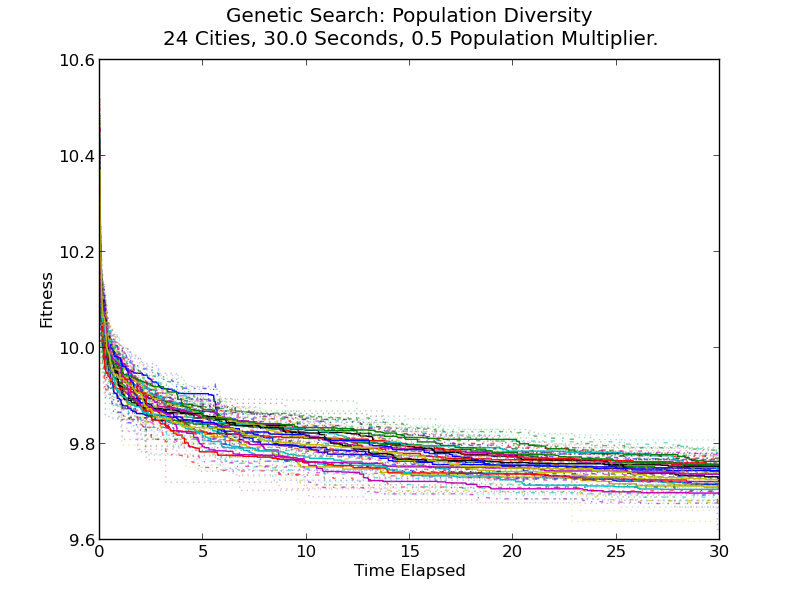
\includegraphics[width=1\textwidth]{../Example_Output_Images/24_cities/30_seconds/populationDiversity_05_populationMuliplier.png}
\end{figure}
The mean is representated as a solid line. The mean $\pm\sigma$ is represented as a dash-dotted line with alpha 0.7 of the same color. The extrema are represented as a dotted line with alpha 0.3 of the same color.
$ $


\newpage
$ $
\newpage
\begin{figure}[t]
  \centering
    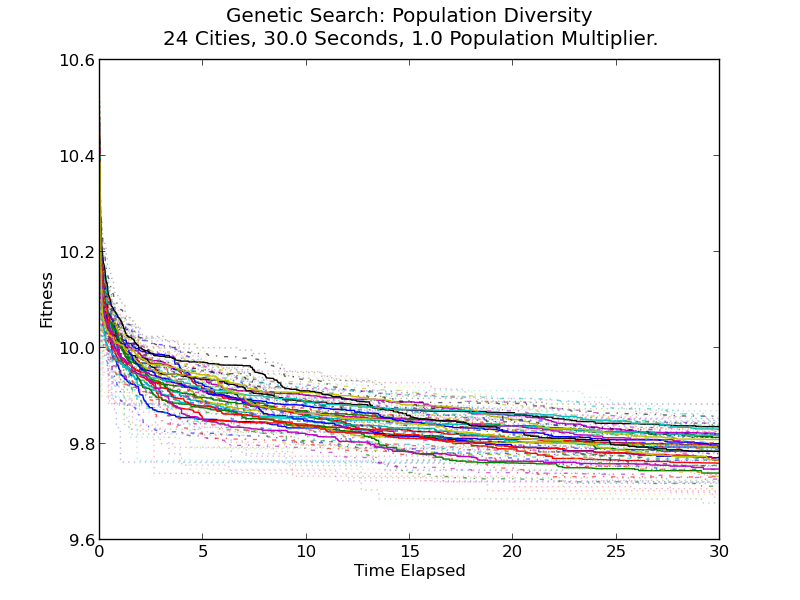
\includegraphics[width=1\textwidth]{../Example_Output_Images/24_cities/30_seconds/populationDiversity_10_populationMuliplier.png}
\end{figure}
The mean is representated as a solid line. The mean $\pm\sigma$ is represented as a dash-dotted line with alpha 0.7 of the same color. The extrema are represented as a dotted line with alpha 0.3 of the same color.
$ $


\newpage
$ $
\newpage
\begin{figure}[t]
  \centering
    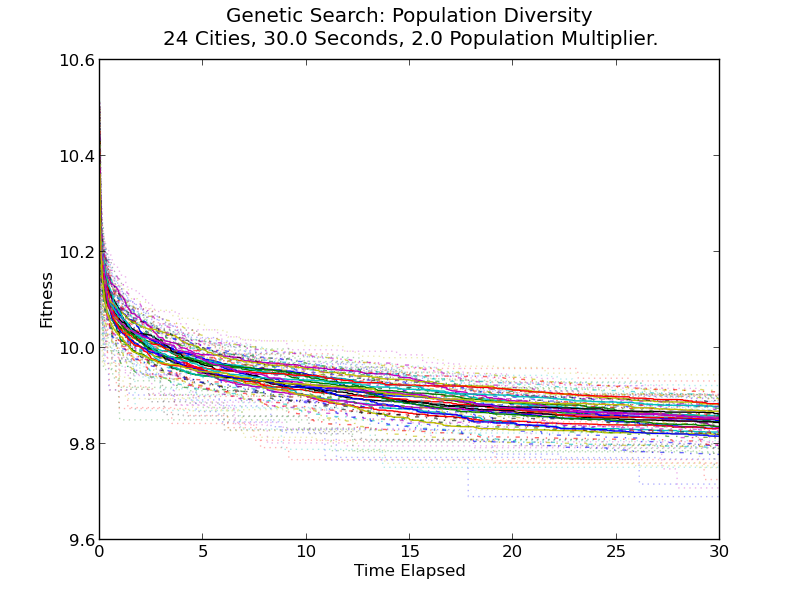
\includegraphics[width=1\textwidth]{../Example_Output_Images/24_cities/30_seconds/populationDiversity_20_populationMuliplier.png}
\end{figure}
The mean is representated as a solid line. The mean $\pm\sigma$ is represented as a dash-dotted line with alpha 0.7 of the same color. The extrema are represented as a dotted line with alpha 0.3 of the same color.
$ $

\end{document}
